~
\newpage
\section{Background on Climate Change \& Ambient Air Pollution}

\subsection{The Earth is Warming (and it's Our Fault)}

In its most recent report, the United Nations' Intergovernmental Panel on Climate Change (IPCC) states:
\begin{quote}
``It is unequivocal that human influence has warmed the atmosphere, ocean and land. Widespread and rapid changes in the atmosphere, ocean, cryosphere and biosphere have occurred." \citep{ipcc1_summary}
\end{quote}
This statement, which follows from possibly the single largest scientific endeavor in human history, is the first critical piece in the climate change story. Before examining why we know that human influence, particularly the burning of fossil fuels, is responsible for the observed warming, we begin by addressing the fundamentals of our current climatic situation. 

We are most familiar with weather, the day-to-day changes in temperature, precipitation, cloud cover, and severe storms. These changes are easy enough to notice by just going outside or looking the window. Climate is a long-run measurement that sizes up weather patterns. In our everyday lives, changes in the climate are much more difficult to detect. Long-run averages of the weather do not exist for anyone to simply look out a window and notice. Fortunately there is data on the day-to-day weather, meaning that with this data, anyone can calculate simple averages of temperatures and look at how climate has changed in even just the last twenty years. To the statistician, weather is a random variable drawn from a distribution, while climate is the moments of this distribution \citep{auffhammer2018quantifying}. 

\begin{figure}
\centering
\caption{The Climate is Warming \citep{ipcc1_summary}\label{ipcc1}}
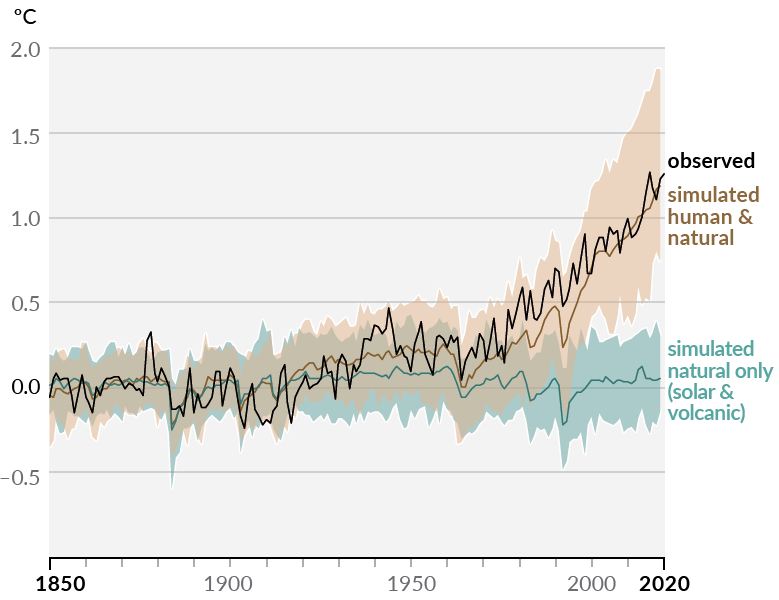
\includegraphics[width=0.6\textwidth]{figures/chapter1_figures/ipcc_fig1.png}
\end{figure}

There is absolutely no question that climate change is occurring. The black line in Figure \ref{ipcc1} displays the change in global temperatures since 1850. The average global surface temperature of the 21st century is 0.99$^\circ$C warmer than the global surface temperature from 1850 to 1900 \citep{ipcc1_summary}. While finding global temperatures is more complicated than a simple average, refuting that the planet is warming amounts to questioning whether or not thermometers actually measure the temperature. The Earth is warming, and even though we cannot go outside and immediately see this, it is still an empirical reality. 

There also no question that climate change is driven primarily by human activity. The tan series in Figure \ref{ipcc1} are simulated results using both human and natural drivers of climate, and the green series are simulated results using only natural drivers of climate. These simulations comes from leading climate models which are heavily reviewed by the scientific community. Natural factors alone cannot explain the rise in global temperatures. Only when we incorporate the impact of humans into climate models does the observed warming make any sense. 

As intelligently crafted as these climate models are, they are remarkably complex. The complexity of these models makes it difficult to understand why the scientific community knows humans are responsible for the recent climate change. Before looking at how scientists attribute the changes in the climate to different factors that have the potential to influence climate, first we look at the possible causes for the climate to change. 

Climate does not change without reason. The energy that warms the Earth and controls the climate comes from the Sun. The Sun covers half of the Earth in radiation at any given time. The atmosphere and Earth reflect about 30\% of this radiation back into space. The atmosphere absorbs 19\% of this radiation, and the surface of the Earth absorbs the remaining 51\%. When absorbed by the Earth's surface, the surface emits infrared radiation, or heat. Surface heat accounts for some of the planet's warmth, but most of this actually comes from the atmosphere \citep{csi}. When the surface emits infrared radiation, this moves out into the atmosphere. Certain particles sometimes absorb this infrared radiation and send it back to the surface. We call these particles \emph{greenhouse gasses}. Greenhouse gases keeps some heat energy from leaving the planet, similar to how a blanket keeps some heat from leaving your body. This heat is not inevitably trapped on the planet, but allows the same energy to be reabsorbed by the surface before attempting to leave the atmosphere again.

The planet's global temperature is stable when the radiative energy that coming into the Earth is equal to the radiative energy that the Earth emits back into space. When the radiative energy that comes to Earth is greater than the radiative energy the leaves Earth, then this surplus energy causes warming \citep{noaa}. This imbalance that causes changes in global temperatures is called \emph{radiative forcing} or \emph{climate forcing}.

There are several major factors that impact radiative forcing: solar irradiation, volcanic eruptions, land use, aerosols, and greenhouse gases \citep{SINGH202179}. \emph{Solar irradiation} refers to the power the Sun gives to the Earth on a per unit of land basis (W/m$^2$). One important factor affecting solar irradiation is the Earth's orbit and rotation. The Earth rotates on a 23.5$^\circ$ axis currently, but over the course of millennia, the tilt of this axis changes. This change in rotation and the subsequent climatic changes are known as the Milankovitch cycles. These cycles also incorporate slight changes in the Earth's orbit that make it more elliptical, bring the planet closer to the Sun during certain periods. While this does affect climate, it does so over the course of thousands of years rather than decades. Other fluctuations from the Sun have the potential to create radiation forcing and changes in the climate over somewhat shorter periods of time. For instance, reduced solar output is a leading explanation of the period of cooler climate in Europe and North America from the early 14th century to the early 19th century, an event known as the Little Ice Age \citep{little_ice}.

Land use, volcanic eruptions, and aerosols affect the planet's \emph{albedo}, the reflectivity of the planet. Recall that the Earth reflects about 30\% of the radiation from the sun. This percentage can change based on the presence of reflective and absorbent features on the surface and in the atmosphere. Some of this reflection occurs at the Earth's surface. White ice reflects radiation, while the black pavement of roads absorbs the Sun's radiation, emitting back the heat or infrared radiation. Agricultural land is generally more reflective than dark forests. Changes in land use like these can affect how much energy the surface absorbs or reflects, and consequently change the planet's albedo and climate. 

Another way to change the Earth's albedo and climate is through aerosol concentrations. Aerosols are small solid or liquid particles in the atmosphere that are can influence cloud cover and the Earth's albedo. Around 90\% of all aerosols in the atmosphere come from natural sources including dust, sea salt, and  wildfire ash. Humans emit the remaining 10\% of aerosols. Burning coal releases sulfur dioxide and driving cars releases fine particulate matter, both aerosols. Aerosols affect climate in two ways: (1) the direct effect of either absorbing or reflecting radiation in the atmosphere, and (2) cloud formation \citep{gfdl}. Most aerosols reflect light and have a cooling effect, with the notable exception of black carbon. Black carbon absorbs light and can be particularly destructive if it coats glaciers, turning these reflective surfaces black. This is the direct effect of aerosols. The second, indirect effect of aerosols is in the creation of clouds. Clouds require aerosols in order to form. Additional aerosols in the atmosphere make cloud formation easier and can even lengthen the lifespan of a cloud. This additional cloud cover reflects radiation and keeps the surface cooler. Unfortunately many common aerosols like sulfur dioxide are dangerous for human health and create acid rain in large concentrations. 

Volcanic eruptions can also influence the planet's albedo. It is true that volcanic eruptions emit greenhouse gases like carbon dioxide. However, volcanic greenhouse gas emissions are less than one percent of all anthropogenic emissions \citep{usgs, gerlach2011volcanic}. The suggestion that higher concentrations of carbon dioxide in the atmosphere are the result of volcanic eruptions rather than human activity is utterly false. Volcanic eruptions can often have a cooling effect on the climate (negative radiative forcing). These eruptions send large quantities of sulfur dioxide, an aerosol, into the troposphere. This creates large, and long-lasting clouds that reflect solar radiation and raise the Earth's albedo. 

\begin{figure}
	\caption{Current Carbon Dioxide Concentrations are Unprecedented \citep{noaa1} \label{noaa1}}
	\centering
	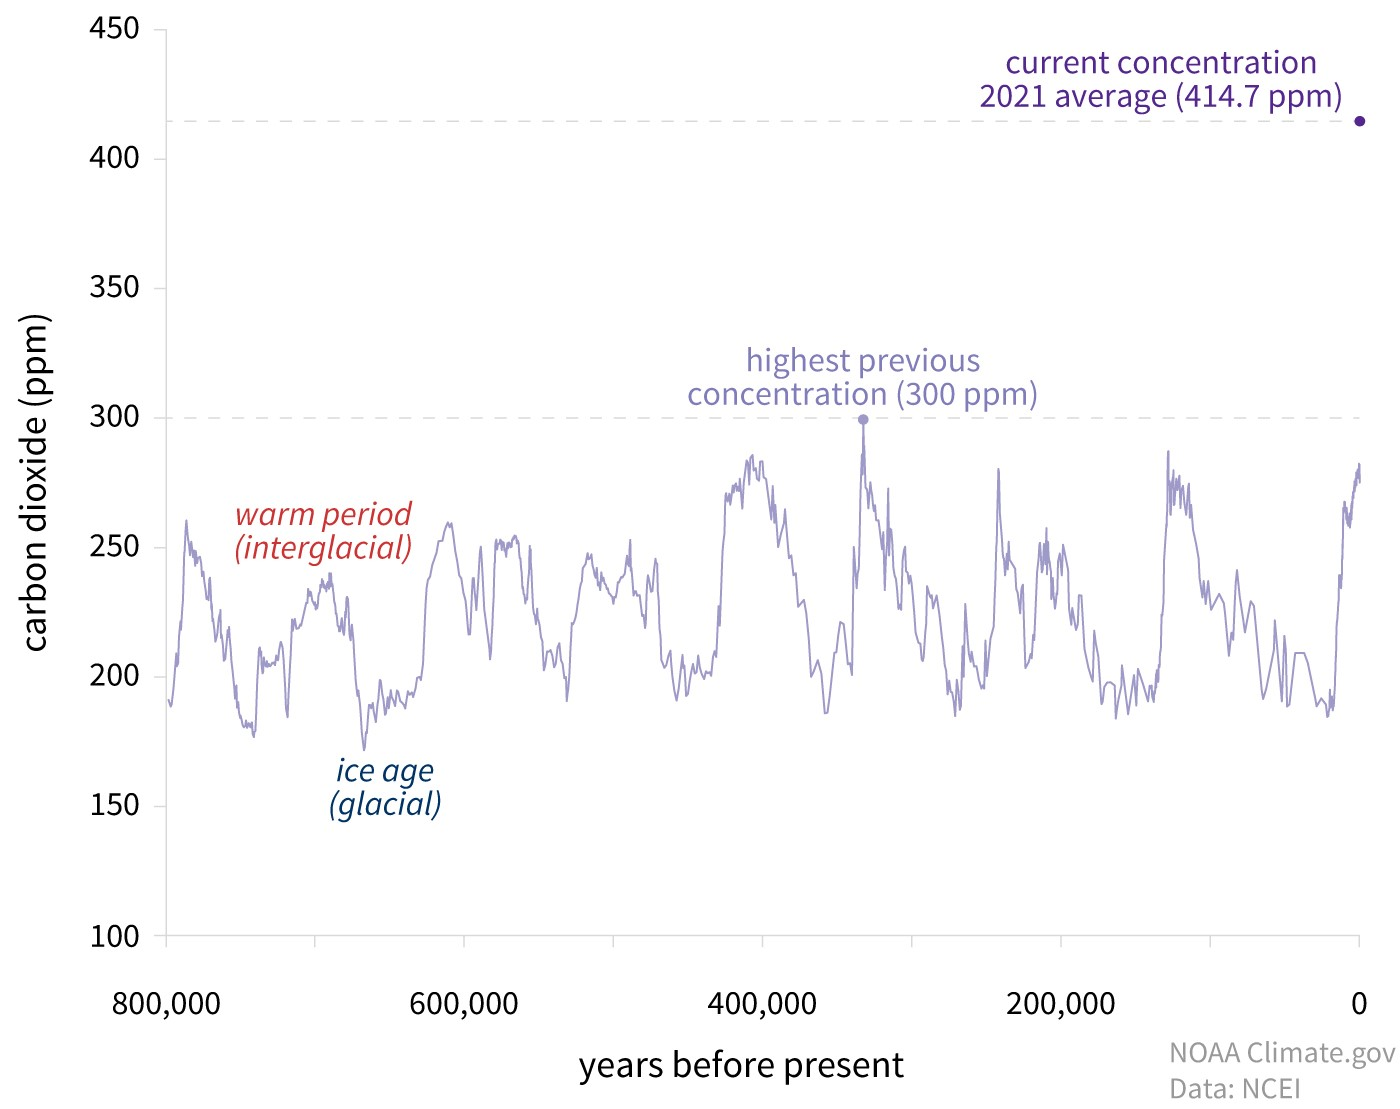
\includegraphics[width=0.7\textwidth]{figures/chapter1_figures/co2_noaa.jpg}
\end{figure}

Lastly, greenhouse gases can create radiative forcing. Higher concentrations of greenhouse gases make it more likely that any infrared radiation emitted on the planet's surface will be re-absorbed by the atmosphere and continue to heat the surface. The most important and common greenhouse gas is water vapor. Water evaporates from the surface, enters the atmosphere, absorbs heat from the planet, and keeps this heat around the surface. We know from the water cycle that the quantity of water vapor in the atmosphere is a function of the current temperature. For water to evaporate, it requires some external warming. For this reason we do not see radiative forcing from water vapor---any warming that occurs as the result of additional water vapor is attributable to the radiative forcing that caused the there to be more water vapor. Water vapor is an accelerator for the warming effect of other greenhouse gases.

The most recognized greenhouse gas is carbon dioxide or CO$_2$. Carbon dioxide makes up the bulk of all human-induced greenhouse gas emissions and, other than water vapor, is the most prevalent greenhouse gas in the atmosphere. Figure \ref{noaa1} shows the concentration of carbon dioxide in the Earth's atmosphere over the previous hundreds of thousands of years. In all this time, the concentration of carbon dioxide in the atmosphere never exceeded 300 parts per million (ppm). In 2020, the atmospheric concentration of carbon dioxide reached 412.5 part per million. Historically, the increase in carbon dioxide is practically instantaneous, and this result is completely attributable to humans. Natural flucuations have played out for hundreds of thousands of years---what we see today is unprecedented and undoubtedly the result of human activity, not natural causes. Elevated concentrations of greenhouse gases can keep additional infrared radiation around the surface of the Earth, warming the world. The next section takes a closer look at greenhouse gas emissions in the US and globally. 

\begin{figure}
\centering
\caption{Warming is Driven by Human Activity \citep{ipcc1_summary}\label{ipcc2}}
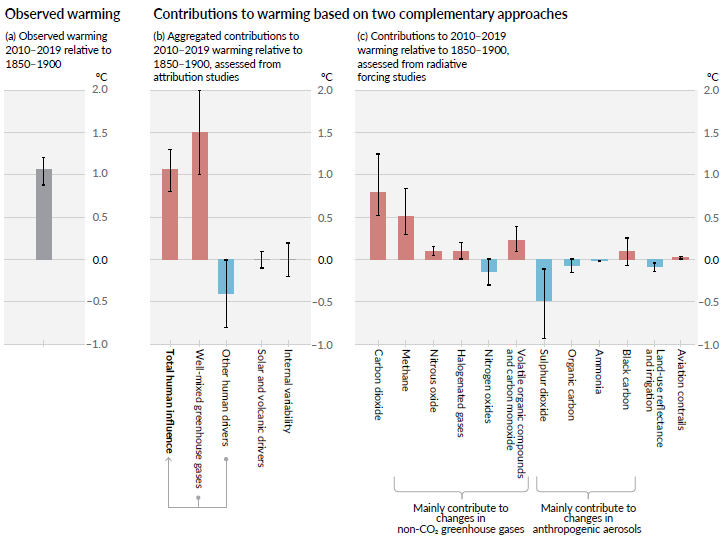
\includegraphics[width=\textwidth]{figures/chapter1_figures/ipcc_fig2.png}
\end{figure}

These various sources, solar irradiance, land use, aerosols, volcanic eruptions, and greenhouse gases, represent a comprehensive list of the factors that could possibly change global temperatures like we have seen them change. From here, scientists can measure how each of these factors have changed over the period we have seen warming. Incorporating some physical constants, researchers calculate the radiative forcing of each of these factors. Figure \ref{ipcc2} displays the results of these radiative forcing studies. This makes it remarkably clear that humans are responsible for climate change. 

Natural radiative forcing from solar drivers, volcanic activity, and internal variability is not perceptible. Historically, this is not surprising. The planet has never warmed so quickly---why would natural forces suddenly cause warming unlike any other time in history? Instead we see that warming is attributable to increases in greenhouse gases like carbon dioxide, methane, nitrous oxide, and others. This warming is partially offset by increasing concentrations of aerosols. Furthermore, we know that humans are responsible for the large increases in these greenhouse gases. We call the climate change caused by humans, rather than natural forces, \emph{anthropogenic climate change}.

If we are not convinced by the calculations of scientists and researchers, observational evidence can still demonstrate the human-origins of climate change. The planet is warming, but not quite the entire planet. The lowest level of the atmosphere that humans inhabit has warmed, but the upper layers of the atmosphere that absorb radiation from the Sun have not \citep{C2ES}. If climate change was the result of some change external to the Earth, then the stratosphere would warm as well. Without any warming in the stratosphere, we know that the warming must occur from activity on the Earth's surface. Natural activities on the surface like volcanic eruptions cannot account account for changes in temperature. These factors have largely remained unchanged over the period of warming we have already encountered, and often make such small contributions to shifts in global climate that we cannot seriously attribute climate change to these factors. Simple deduction leaves human activity as the culprit of the climate crisis. The Fourth National Climate Assessment makes the summation of all these scientific observations clear:
\begin{quote}
``Global average temperature has increased by about 1.8°F [1.0$^\circ$C] from 1901 to 2016, and observational evidence does not support any credible natural explanations for this amount of warming; instead, the evidence consistently points to human activities, especially emissions of greenhouse or heat-trapping gases, as the dominant cause." \citep{nationalar4}
\end{quote}


\subsection{Greenhouse Gas Emissions: Structure \& Trends}

Anthropogenic greenhouse gas emissions drive climate change. Carbon dioxide, methane, and nitrous oxide dominate greenhouse gas emissions in the US and globally. Florinated gases, also called F-gases, make up a non-negligible proportion of greenhouse gas emissions in the US, and are growing at an alarming rate.

Not all greenhouse gases are created equal. Some greenhouse gases remain in the atmosphere longer than others and absorb more infrared radiation from the Earth than others. Greenhouse gases may also react and create different greenhouse gases in the atmosphere, which themselves can have different warming effects. To improve the accounting of greenhouse gases, researchers standardize the varied warming effect of these greenhouse gases through a measure called global warming potential (GWP). GWP measures the warming effect of other greenhouse gas emissions relative to the warming effect from a ton of carbon dioxide. For instance, in the IPCC's 5th Assessment Report, methane has a GWP of 28, meaning that a ton of methane emissions has the same warming effect as 28 ton of carbon dioxide. This metric then leads to carbon dioxide equivalent emissions, a standard unit of account for different greenhouse gas.

\begin{table}
\centering
\caption{Global Warming Potential (GWP) by Greenhouse Gas \label{gwptable}}
\begin{tabular}{l c C{4cm} C{4cm}}
	\hline
	& & \multicolumn{2}{c}{IPCC Calculated GWP  over 100 Years}\\	
	\cline{3-4}
	Gas Name & Chemical Formula & Fourth Assessment Report & Fifth Assessment Report \\ 
	\hline
	Carbon dioxide & CO$_2$ & 1 & 1 \\
	Methane & CH$_4$ &25 & 28 \\
	Nitrous oxide & N$_2$O & 298 & 265\\
	HFC-134a & CH$_2$FCF$_3$ &1,430 & 1,300\\ 
	HFC-23 & CHF$_3$ & 14,800 & 12,400 \\
	Nitrogen trifluoride & NF$_3$ & 17,200 & 16,100\\
	Sulfur hexafluoride & SF$_6$ & 22,800 & 23,500\\
	\hline
\end{tabular}\\
\smallskip

\raggedright \footnotesize
Original data from \cite{forster2007changes} and \cite{ipcc_ar5_forcing}. Table adapted from \cite{gwp_table}.
\end{table}

Table \ref{gwptable} lists the GWP for the most common greenhouse gases and a handful of F-gases as calculated under the IPCC's Fourth and Fifth Assessment Reports. Carbon dioxide is always one because it is the standard unit. Methane has a shorter atmospheric lifespan than carbon dioxide, but absorbs much more energy during this time. The agriculture industry accounts for the largest share of methane emissions, followed closely by the mining and processing of fossil fuels.\footnote{\url{https://www.epa.gov/ghgemissions/overview-greenhouse-gases}} Nitrous oxide emissions occur almost entirely from agriculture, particularly from the application of fertilizers and other soil management practices. These emissions linger in the atmosphere longer than methane and absorb heat better than carbon dioxide. The IPCC's  latests estimates indicate one ton of nitruos oxide equates to 265 tons of carbon dioxide. F-gases like HFC-134a (the most common hydroflorocarbon in the atmosphere), HFC-23, nitrogen trifluoride, and sulfur hexafluoride are rare. These gases emerged to replace chlorofluorocarbons following the Montreal Protocol. While these gases do not have quite the same ozone-destroying effect of their predecessors, they can have huge GWP in even small quantities. They tend to remain in the atmosphere for a much longer time and absorb far more energy than more common greenhouse gases. For this reason, F-gases are also often called high GWP gases.

\begin{figure}
\caption{US Greenhouse Gas Emissions 1990--2019\label{ghg1}}
\centering
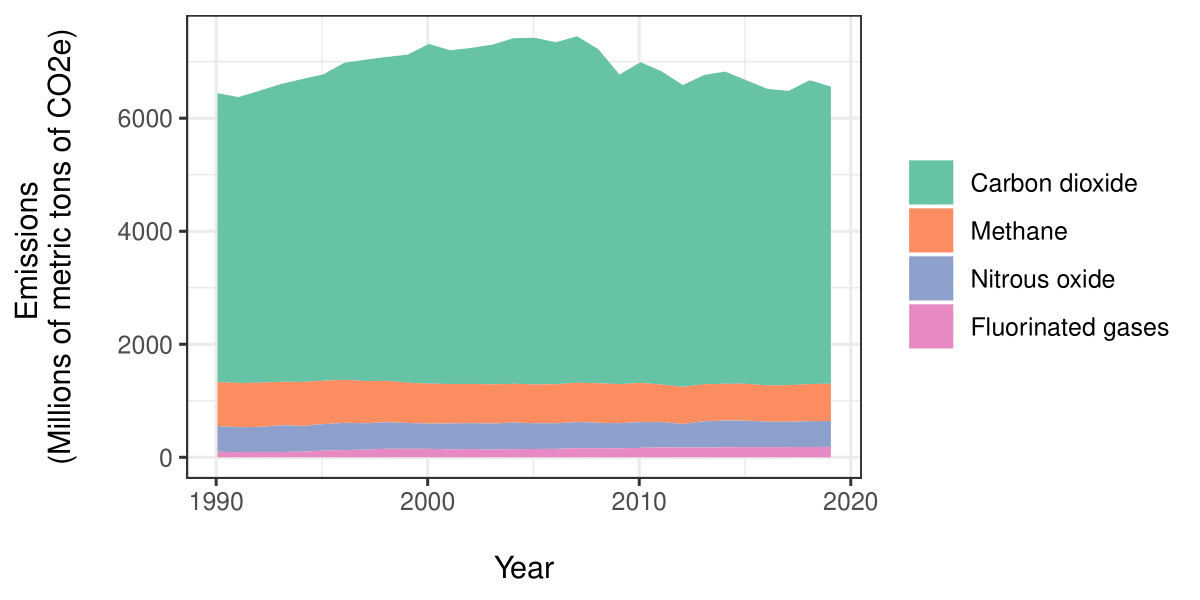
\includegraphics[scale=1]{figures/chapter1_figures/ghg_stacked.png}
\end{figure}

When we put all anthropogenic emissions into a common measurement, carbon dioxide equivalent, then we can compare greenhouse gas emissions and accurately evaluate the composition of greenhouse gases and the threat of certain gases relative to others. Figure \ref{ghg1} plots total greenhouse gas emissions (in millions of metric tons of carbon dioxide equivalent, CO$_2$e) in the US from 1990 to 2019 by the offending greenhouse gas. First, US greenhouse gas emissions have fallen over the past ten years. Second, it is clear why there is so much emphasis on carbon dioxide. Carbon dioxide makes up a clear majority of all anthropogenic greenhouse gas emissions in the US. Most of the recent reductions in greenhouse gas emissions are attributable to falling carbon dioxide emissions. Although they still make up just sliver of emissions, F-gases have seen the most growth over the period, up 86.3\%. 

\begin{figure}
\caption{US Greenhouse Gas Emissions by Economic Sector 1990--2019 \label{ghgeconomic}}
\centering
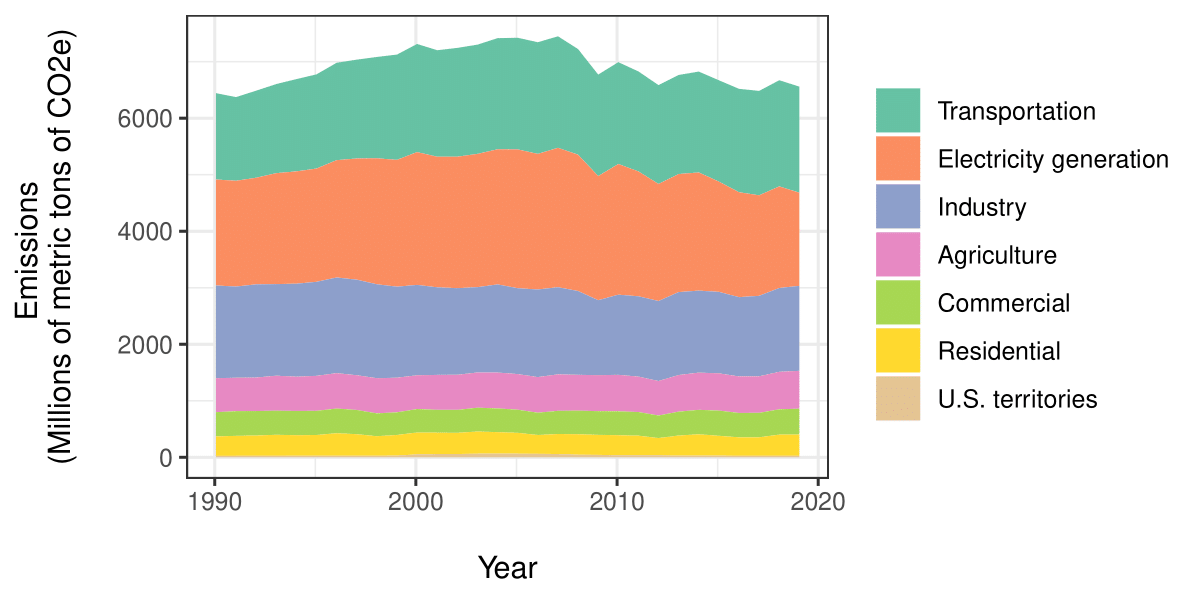
\includegraphics[scale=1]{figures/chapter1_figures/ghg_economic.png}
\end{figure}

Where then are these greenhouse gases coming from? One way to answer this question is by looking at greenhouse gas emissions by economic sector. Figure \ref{ghgeconomic} plots the greenhouse gas emissions of major US economic sectors in carbon dioxide equivalent from 1990 to 2019.  The emissions reductions from electricity generation and industry have driven the most recent decline in greenhouse gases. Transportation has consistently been the largest source of emissions, making up 28.6\% of all US greenhouse gas emissions in 2019. Electricity generation makes up a slightly smaller share with a clearer path to zero emissions through the expansion of renewable electricity generation and other low-carbon intensity fuel sources. Industrial greenhouse gas emissions have fallen by just about 8\% since 1990, and 22.9\% of all US emissions were from industry in 2019. The agriculture industry contributed 10.2\% of all US emissions in 2019. Commercial and residential emissions occur mostly from burning fossil fuels to heat buildings and homes. Together, these accounted for 12.7\% of all emissions in 2019. 

\begin{figure}
\caption{US Greenhouse Gas Emissions by Inventory Sector 1990--2019}
\centering
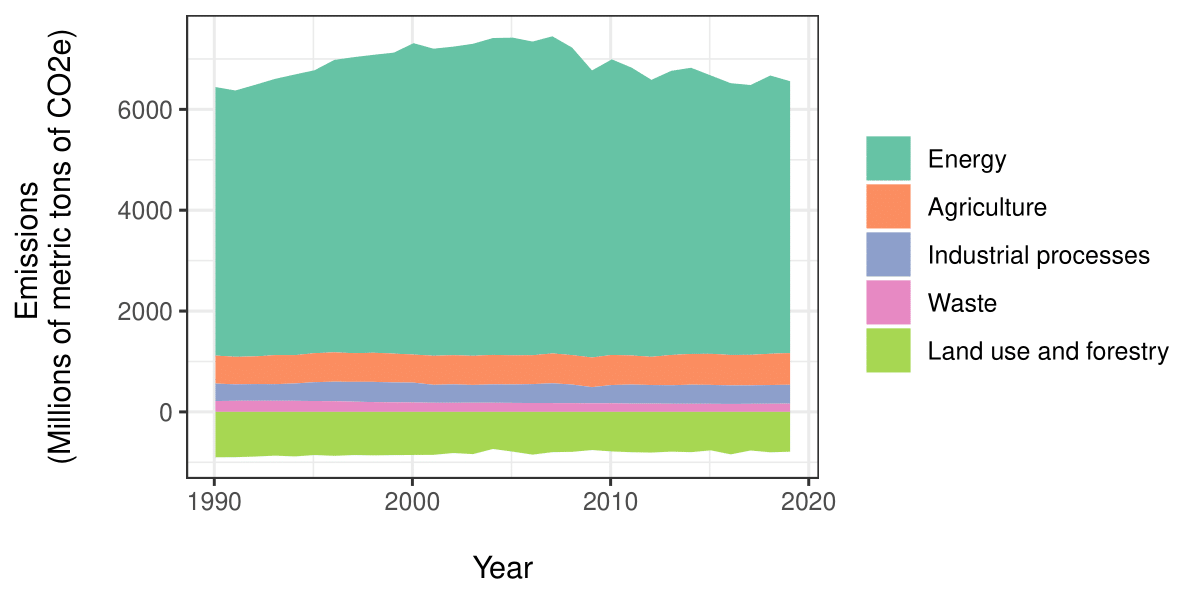
\includegraphics[scale=1]{figures/chapter1_figures/ghg_inventory.png}
\end{figure}

The US also reports greenhouse gas emissions by inventory sector, which considers the physical sources that create and remove emissions. This can be more useful than looking greenhouse gases by economic sector if different economic sectors create emissions for similar reasons. Indeed, we see that energy generation commands the majority of greenhouse gas emissions across economic sectors. Energy makes up 82\% of gross greenhouse gas emissions in the US. This is driven by the burning of fossil fuels, releasing carbon that was trapped in the ground into the air. Agriculture and waste both make meaningful contributions, mostly through methane and nitrous oxide emissions. Hydroflorocarbons and other high GWP gases are responsible for a considerable portion of emissions that occur during industrial processes. The EPA also reports data on the nations carbon sink. Carbon dioxide cycles naturally through the environment, emitted into the atmosphere by decomposing organic matter and reabsorbed by plants life. This natural carbon sequestration creates the carbon sink. Forestry and other plant life remove emissions from the air and store them, a flow of greenhouse gas emissions out of the atmosphere. For the US to reach net zero greenhouse gas emissions, this carbon sink must be equivalent to all other greenhouse gas emissions. 

\begin{table}
\caption{US Electricity Generation by Source \label{ele_gen_source}}
\centering
\begin{tabular}{l C{3cm} C{3cm}}
\hline \hline
Energy source & Billion kWh &	Share of total \\ 
\hline 
Fossil fuels & 2,427 & 60.6\% \\
\qquad Natural gas &	1,624	& 40.5\% \\
\qquad Coal & 773 & 19.3\%\\
\qquad Petroleum	& 17 & 0.4\% \\
\qquad Other gases & 11& 0.3\% \\
Nuclear & 790	& 19.7\% \\
Renewables & 792 & 19.8\% \\
\qquad Wind & 338 & 8.4\%\\
\qquad Hydropower	& 291 &	7.3\% \\
\qquad Solar & 91 & 2.3\% \\
\qquad Biomass	& 56 & 1.4\% \\
\qquad Geothermal & 17 & 0.4\% \\
Other sources & 8 & 0.2\% \\
Total: All sources	& 4,007  & ---\\
\hline \hline
\footnotesize \raggedright Data from \cite{eia_report1}.
\end{tabular}
\end{table}

With electricity generation and energy broadly making up such a considerable portion of US greenhouse gas emissions, it is important to understand the composition of electricity generation by fuel source in the US. Table \ref{ele_gen_source} shows the fuels that drive US electricity generation. Fossil fuels make up the majority of electricity generation with 60.6\% of all electricity coming from fossil fuels. Natural gas is the single largest fuel source for US electricity generation, with more electricity from natural gas than the next two most common fuels (nuclear and coal) combined. Natural gas burns much cleaner than coal; coal emits 95.74kg of carbon dioxide per million BTUs on average while natural emits 52.91kg of carbon dioxide per million BTUs.\footnote{British thermal units (BTUs) measure thermal energy. One BTU is the amount of heat energy required to warm one pound of water by one degree Fahrenheit. \url{https://www.eia.gov/environment/emissions/co2_vol_mass.php}} Still, Figure \ref{ghgeconomic} shows that despite the low emissions intensity of natural gas relative to other fossil fuels, it is still a fossil fuel that produces significant emissions. Fuels with low carbon intensities, like nuclear and renewables, make up the remainder of electricity generation, around 40\% of all US generation.

Climate change and excess greenhouse gas emissions might be a much simpler problem to address if they were unique to the US. They are global problems, and while the US is a major emitter of greenhouse gases, it is not the only nation with significant emissions. Figure \ref{global_ghg} shows the greenhouse gas emissions by country from 1990 to 2016. China is the largest producer of greenhouse gases, followed by the US. India and the European Union currently put similar quantities of greenhouse gases in the atmosphere, but are trending in opposite directions. As India develops, its emissions are growing, while Europe's emissions are falling. We see here that just a few countries, particularly the US and China, make up a significant portion of all greenhouse gas emissions. In these countries, emissions reductions are especially important. 

\begin{figure}
\caption{Global Anthropogenic Greenhouse Gas Emissions 1990--2016 \label{global_ghg}}
\centering
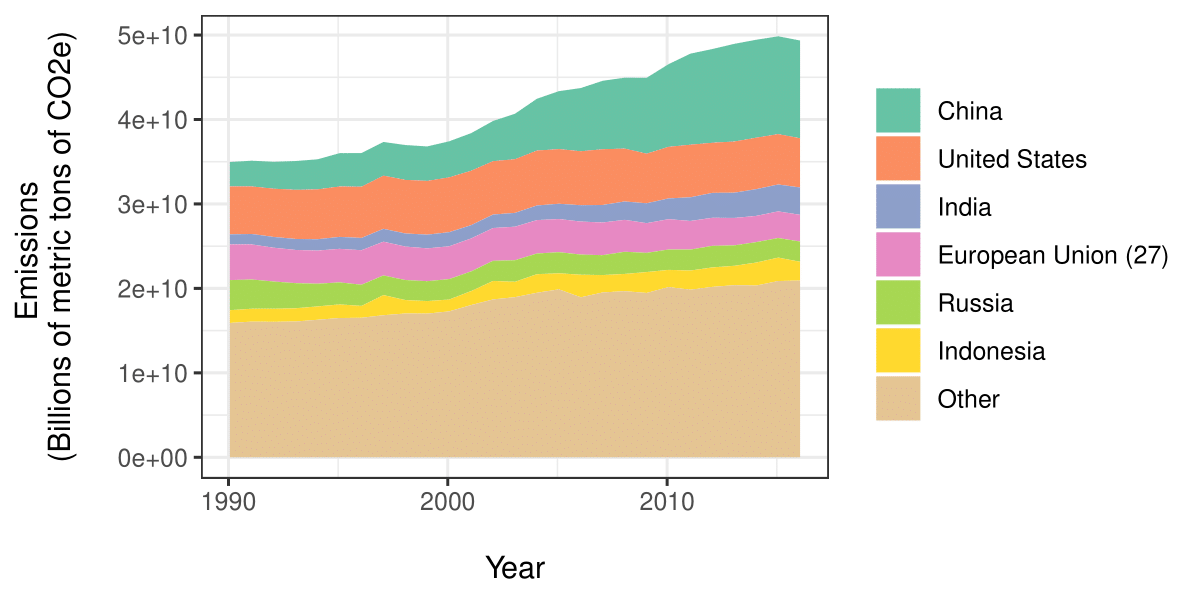
\includegraphics[scale=1]{figures/chapter1_figures/ghg_international.png}
\end{figure}

Although the US is a major contributor to global greenhouse emissions, it is not the largest (second place, woohoo). When we consider greenhouse gas emissions in per capita terms though, the situation in the US seems even more imperiled. Figure \ref{global_ghg_cap} looks at greenhouse gas emissions per capita for the leading greenhouse gas contributors. The US far outpaces other developed nations. Notably, the US has more than double the greenhouse gas emissions per capita as China. The US stands out on the global stage as in terms of wealth, size, and apparent inability to reduce its greenhouse gas emissions.

\begin{figure}
\caption{2016 Greenhouse Gas Emissions per Captia of Leading Emitters \label{global_ghg_cap}}
\centering
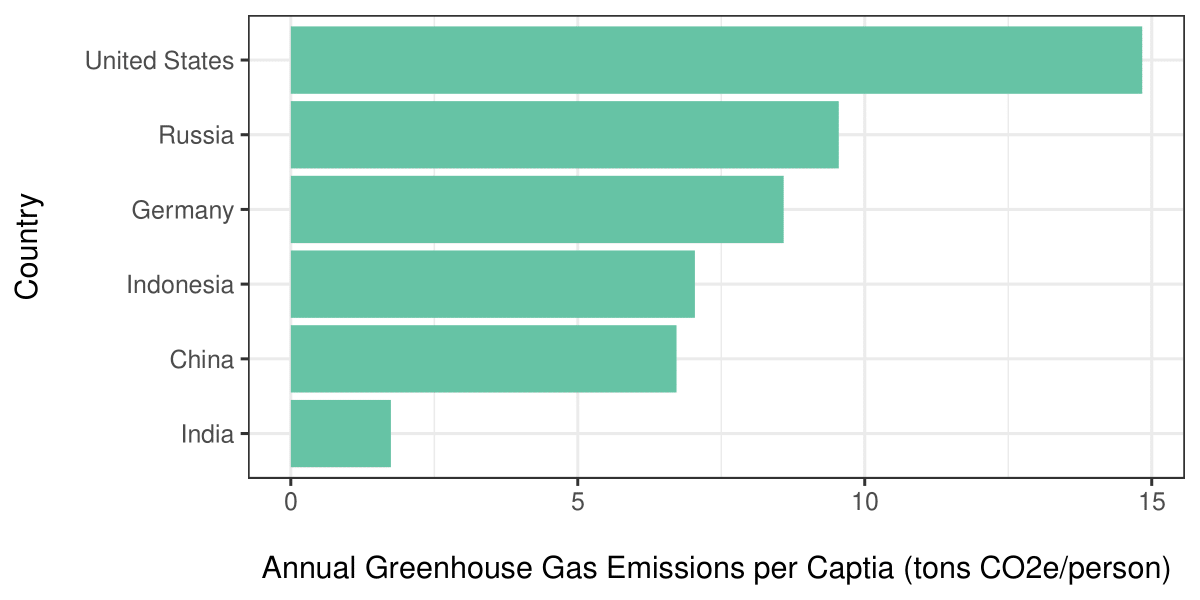
\includegraphics[scale=.9]{figures/chapter1_figures/ghg_cap.png}
\end{figure}


\subsection{The Impacts of Climate Change}

The previous sections have demonstrated that human activity, particularly the burning of fossil fuels, is responsible for climate change. Before we start designing policy to reduce greenhouse gas emissions, we first need to understand how climate change affects us today and could affect us in the future. In this section, we discuss some of the major impacts of climate change.

First though, we should discuss how we estimate future damages from climate change. 

The overarching approach 

Before we can estimate how climate change will affect the world in the future, we have to start with assumptions about what the world will look like in the future. Given this, we then 






The goal of climate impact studies is to estimate how emissions today and in the future will lead to a climatic scenario and then estimate how that climatic scenario will ripple through different ecosystems, communities, and economies. Economists often take this a step or two further, and try to put all of the costs (and benefits) of climate change into economic terms and then tie these prices into present terms. This gives the foundation for the the social cost of carbon [CITATION, https://www.rff.org/publications/explainers/social-cost-carbon-101/]. For our present purposes we do not need to relate all of these impacts back into prices, so we will omit a more detailed description of the social cost of carbon for now. 

The inputs to these climate impact models are known as emissions pathways. Despite the name, emissions pathways do not truly map out different emissions scenarios, but different concentrations of greenhouse gases alongside certain socioeconomic assumptions. A simplified emissions pathway might assume a certain time series of greenhouse gas concentrations, human population, and GDP over the century. The Intergovernmental Panel of Climate Change (IPCC) has standardized two collections of emissions pathways: Representative Concentration Pathways (RCPs) and Shared Socioeconomic Pathways (SSPs).\footnote{Often you might see something such as ``RCP$_{4.5}$" or ``SSP$_{8.5}$." The numeric subscript indicates the amount of radiative forcing the emissions scenario creates by 2100. For instance, RCP$_{4.5}$ will lead to 4.5 W/m$^2$ of radiative forcing---a measure of the average energy absorbed by the planet. Similarly, SSP$_8.5$ creates 8.5 W/m$^2$ by 2100, and is often used as the ``do nothing" response to cliamte change [CITATIONS, AR6 SPM]} Climate models then assume these scenarios and map out what the climate looks like over the course of the century using these 

% - Something about General Circulation Models (GCMs?)?
% - What are the CMIP things?

Process-based models suffer in in important ways. First, they are computationally intensive. 



While these process-based models create the backbone of impact estimates, economists often opt to use simpler method for mapping climatic outcomes to quantitative impacts called damage functions. Damage functions are reduced-form estimations of the relationship between climate variables (e.g. average surface temperatures) and impact variables of interest (e.g. mortality rates). That is, damage functions do not attempt to explain the complex systems that give rise to these damages and focus instead on just explaining aggregate impacts. For instance, [CITATION] create straightforward damage functions for the US by using process-based impact models to generate estimates of climate change impacts (in monetary terms) under a variety of climate scenarios. Then they use OLS to estimate the relationship between surface temperature measurements and the monetary value of climate change impacts. The estimated model is a damage function, mapping changes in surface temparatures to impacts. Damage functions like this and many others provide useful tool in a variety of applications, especially in calculating the social cost of carbon. 

\cite{auffhammer2018quantifying} notes that perhaps the greatest difficulty in using damage functions to map climatic scenarios into physical impacts is accounting for adaptation. Although it would be much easier to assume that people and businesses . \cite{auffhammer2018quantifying} uses the example of an air conditioner. Suppose we are interested in the impact of a changing climate on electricity use. We expect there to be more hot days, meaning that people will run their air conditioners more frequently and use more electricity to do so. This response on the intensive margin is measurable; we have the data to estimate how people use their air conditioners differently when it is warmer outside. The extensive margin cannot be realiably measured. 
We do not have reliable measurements for how many more people will purchase and use air conditioners after decades of sustained warming.\footnote{A promising but limited approach to studying climate change adaptation is by estimating how people have adapted to climate changes in the past. For instance, [CITATION, Drunkenmiller] are using historical aerial photographs of Western Africa to study land use and migration changes that occurred as a result of drought during the mid-twentiwth century.}

Admittedly, there is a considerable amount we still do not know about the impacts of climate change. Truthfully, we are not exactly sure how the estimated 3.3 to 3.6 \emph{billion} people who are highly vulnerable to climate change will adapt [CITATION]. Will hundreds of millions of people living in some of the most impoverished corners of the planet seemlessly migrate en masse to places with more hospitable climates over the course of just a few decades? 

What we do know is that today, our best estimates indicate that the impacts of climate change are frightening. 

In the preceeding subsections, we look at the

The IPCC outlines five major ``reasons for concern" regarding climate change:
\begin{enumerate}
	\item Unique and threatened systems
	\item Extreme weather events
	\item Distribution of impacts
	\item Global aggregate impacts
	\item Large-scale singular events
\end{enumerate}
These represent some of the most important risks that we face from climate change. 

% intramarginal vs. extramarginal

\subsubsection*{Unique \& Threatened Systems}

While many systems---both natural and social---face steep challenges from climate change, some of these face complete ruin. Many of the most vulerable systems are endemic. Endemism refers to species, cultures, and resources that are restricted to specific geographic areas. [CITATION] In a changing climate, systems that are tied to specific regions and climates risk extinction if they cannot plausibly adapt. This includes the extinction of species whose habitats are destroyed by climate change, 
the death of indigenous cultures that are highly dependent on the climate, and the destruction of historical artifacts and landmarks. Unfornately in each of these cases, the affected system cannot is unique and we could not replace it for the remainder of human existence. These kind of consequences do not fit well into standard economic understanding of sustainability. \footnote{*Talk about an economic definition of sustainability from Romer, and why it might not be able to capture some of the threats of climate change well.*}


\subsection{The Impacts of Ambient Air Pollution}

\textit{Forthcoming}.


\subsection{A Review of Air Quality Disparities}

\textit{Forthcoming}.



%%%%%%%%%%%%%%%%%%%%%%%%%%%%%%%%%%%%%%%%%%%%%%%%%%%%%%%%%%%%%%%%%%%%
%\subsection{The Impact of Climate Change}
%
%At this point we have covered why we know climate change exists, why we know humans are responsible for climate change, and what the composition of greenhouse gas emissions look like. We have to to justify why anyone should care about climate change though. Here, we take a brief and high-level examination of the impacts of climate change. If I had to summarize the magnitude of climate impact estimates by even just the end of the century, I would probably say that they lie somewhere in between pretty bad to borderline apocalyptic. 
%
%Admittedly, the impacts of climate change on natural ecosystems and society are not understood quite as well as the causes of climate change. This gap in knowledge is closing as we collect new data on the impact of the climate change we have already seen. The IPCC summarizes these impacts in its Fifth Assessment Report in five ``reasons for concern." These reasons for concern relate to:
%\begin{enumerate}
%	\item Unique and threatened systems
%	\item Extreme weather events
%	\item Distribution of impacts
%	\item Global aggregate impacts
%	\item Large-scale singular events
%\end{enumerate}
%
%There are certain physical elements of the natural and built environment that are unique and irreplaceable. Losing these due to climate change poses a significant cost for all future generations. For instance, warming waters threatens coral reefs. With sustained and substantial warming, the world's coral reefs could be permanently destroyed. Many important historical sites are located in low-lying coastal areas threatened by rising sea levels from climate change. Climate change has the power to permanently destroy many of the ecosystems we cherish and other culturally significant creations.
%
%Extreme weather events pose the greatest This includes a greater frequency of severe but short-lived weather events, like tornadoes or monsoons. More concerning is are sustained heat-stress events. As Freddy's mom from iCarly once said, ``when temperatures get too high, the elderly will start to die" (a rather creepy but fitting rhyme). Elevated temperatures can induce cardiovascular events, particularly in vulnerable populations like the poor, elderly, and those who work outside. Sustained events like this can trigger droughts and resulting in famine. Higher humidity can bolster mosquito populations and allow blood-borne infectious disease to spread easier. Extreme and sustained events like these pose serious challenges to public health.
%
%Related to this, impacts tend to fall most severely on populations who are already at the greatest disadvantage. Some of this is simply due to geography. Climate predictions for the African continent are sickening. Much of this is due to adaptation costs. When it is 110$^\circ$F outside, the well off do not just sweat---they run their air conditioners on full blast. This is not true of the global poor, who cannot afford to pay to adapt to rising temperatures, and instead suffer the heat and risk death. 
%
%Global impacts on natural life and the economy are not well understood, but what we know is not reassuring. The economic impacts of climate change will become much more apparent as concentrations of greenhouse gases increases. That is, the economic damages from climate change are increasing at an increasing rate with the concentration of greenhouse gases. There is some additional concern about low-probability, highly dangerous climate change-induced events. 
%
%\begin{figure}
%	\caption{Climate Change Damages by Income \& Climate \citep{carleton2020valuing} \label{cil1}}
%	\centering
%	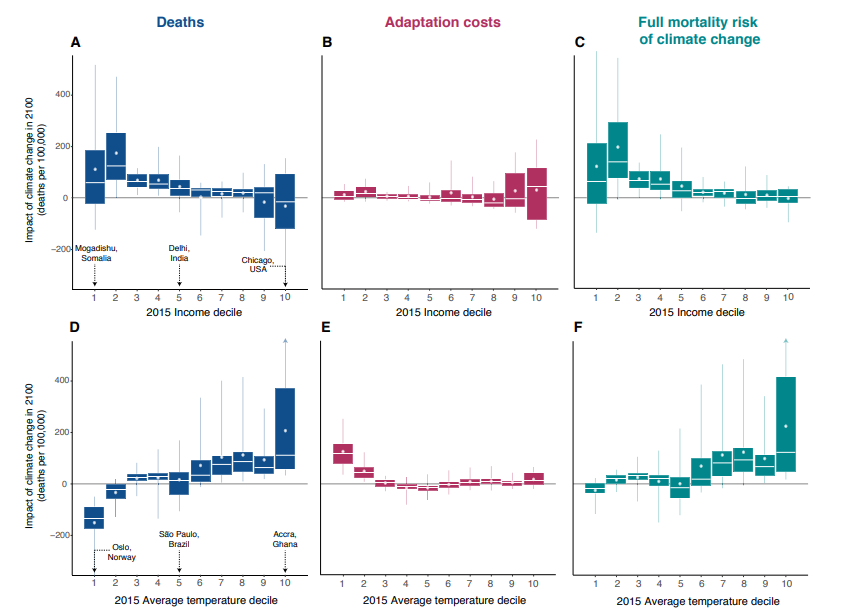
\includegraphics[width = \textwidth]{figures/chapter1_figures/cil_dist.png}
%\end{figure}
%
%\begin{figure}
%	\caption{The Climate Change Mortality Rate \citep{carleton2020valuing} \label{cil2}}
%	\centering
%	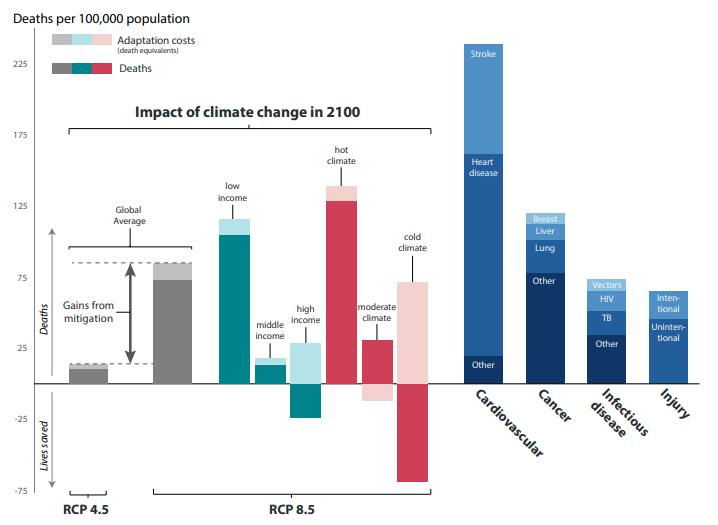
\includegraphics[width = 0.8\textwidth]{figures/chapter1_figures/cil_mortal.png}
%\end{figure}
%
%Figures \ref{cil1} and \ref{cil2} depict estimates of moralities by end of the century from climate change induced events. These summarize many of the most important takeaways from the impacts of climate change. Those who live in poor and warm areas will suffer the most from climate change. The mortality rate from climate change is comparable to the mortality rate of other leading causes of death. Overall, the situation climate change poses by just the end of the century is extremely grim and warrants sweeping action.